\chapter{Предварительно}

Есть в Киеве важнейшее место – Кирилловские высоты. Так условно, краеведами и археологами, называются горы вдоль улицы Кирилловской, она же Фрунзе. Дорога тут была издревле, соединяя Подол с Кирилловским монастырем.

Эта часть книги охватывает не все Кирилловские высоты, а отрезок от Щекавицы по Смородинский спуск, ибо дальше идут еще холмы – это и гора со знаменитыми, описанными в преданиях и былинах, пещерами, где змей жил, и Кирилловский монастырь тоже на горе – так что Кирилловские высоты длятся на север через Куренёвку до Шполянки (бывшие дачи Шполянского).

К пещерам и монастырю мы еще доберемся, пока же посетим юг и середину высот. В ходе повествования я буду привлекать много архивных документов, а также материалы, наработанные неутомимыми исследователями этой местности – Владимиром Бонифатьевичем Антоновичем, Викентием Хвойкой, Кондратом Лохвицким и другими. Добытые ими сведения зачастую буду приводить целиком, ибо они крайне редки и ценны. Других нет и не будет – описанное уничтожено.

Хвойка наиболее полно документировал свои находки, как текстом, так фотографиями и рисунками, хотя всё это даже сейчас, в эпоху оцифровок, составляет труд достать с миру по нитке.

\begin{center}
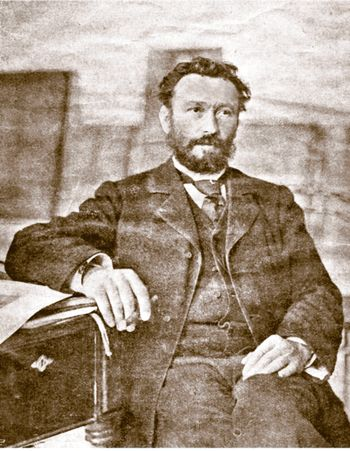
\includegraphics[width=0.68\linewidth]{chast-kirvys/predvaritelno/hvoyka-9x.png}

\textit{Викентий Хвойка, фото конца 19 века.}
\end{center}

Викентий Хвойка (Čeněk Chvojka) родился 21 февраля 1850 года в селе Семин (нынче оно в Чехии, а тогда было в Австро-Венгрии), в крестьянствующей семье обедневших рыцарей. В Праге закончил он коммерческое училище. В 1876 году по неким причинам сбежал в Российскую империю, поселился в Киеве и стал работать учителем. Преподавал немецкий язык, фехтование и рисование. Выращивал новые сорта хмеля, проса и придумывал способы их переработки, о чем писал научные работы. Труды Хвойки на этом поприще были оценены похвальным листом да бронзовой медалью на выставках в Ромнах (1884) и Харькове (1897), серебряной медалью на Парижской сельскохозяйственной выставке (1889) – там его избрали членом Французской национальной сельскохозяйственной, промышленной и коммерческой академии.

Одно время Хвойка обитал под Киевом, в селе Петрушки (Святошинский район), в имении или даче чешской семьи Дефорен. Там у Хвойки был сарай-лаборатория, где ученый работал и хранил всё добро – рисунки, чертежи, медали. В 1890 году сарай сгорел. 

Хвойка наблюдал, как рабочие расчищают пепелище, и заметил, что вместе с землей они бросают лопатами некие стекляшки синего, зеленого, розового цвета. Хвойка отмыл их и показал в Киеве любителям старины. Те определили в находке браслеты времен Киевской Руси. Владелец выручил за них 60 рублей.

Так Хвойка увлекся археологией, в которой сделал для наших краев пожалуй больше, чем все другие археологи, и положил основу многим последующим наработкам. В науке он открыл трипольскую, черняховскую, зарубинецкую культуры, странные сооружения на Старокиевской горе (среди них якобы капище), памятники еще более седой древности, в том числе – Кирилловскую стоянку. Хвойка был одним из основателей Киевского общества древностей и искусств, способствовал созданию Киевского городского музея.

Кажется, Хвойкой двигал не только коммерческий интерес, но и проснувшаяся тяга к познанию давних времен. В 1891 году он писал отцу в Чехию, что ищет в разных местах то, что давно исчезло, особенно «первые следы наших славянских праотцов». Конечно, на раскопки нужны были деньги, и находки отправлялись затем в частные коллекции заказчиков – Терещенко, Ханенко. Копал и за свой счет.

Умер 2 ноября 1914 года – туберкулез. Похоронен на Байковом.

Именем Хвойки названа в Киеве улица, точнее переименована – бывшая Езерская (по фамилии домовладельца) или Новокирилловская. Проходит она четко от железной дороги перпендикулярно к Кирилловской, стыкуясь с нею почти напротив Смородинского спуска. Мало кто знает, что там был один из домов археолога. Прежде туда заходили живший на Кирилловских высотах художник Светославский, археолог и собиратель преданий Ляскоронский, рабочие-землекопы, приносившие свои находки, а также скупщики древностей.

%Еще в 2013 году я написал – вообще всё, что примыкает к основным холмам Кирилловских высот, носит отпечаток какой-то вымороченности. Много зданий, застывших в вечном ремонте. Пешеходов мало, движения почти нет, только ветер гоняет сухие листья. Улица Фрунзе, или Кирилловская, оживляется только ближе к Куренёвке или к своему началу возле Подола. Но летом 2014 года замороженные здания сдали в аренду, вдоль улицы выстроились ряды машин, зашагали люди. Фрунзе будет нашей основной дорогой в путешествии по высотам.

\newpage
\vspace*{\fill}
\begin{center}
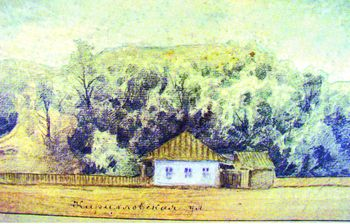
\includegraphics[width=\linewidth]{chast-kirvys/predvaritelno/hv-ris.png}

\textit{Кирилловская улица. Художник Викентий Хвойка.}
\end{center}

\begin{center}
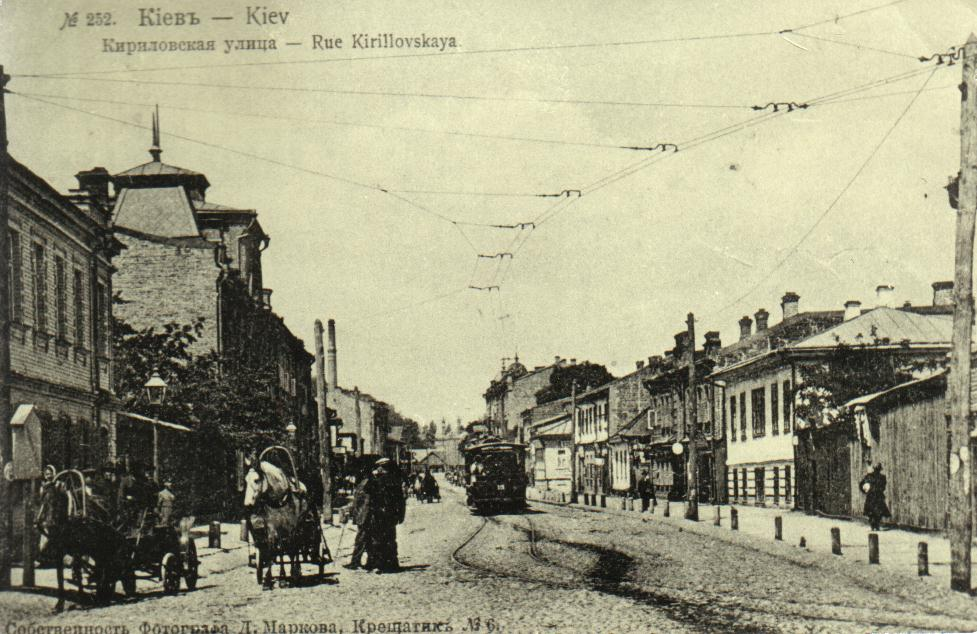
\includegraphics[width=\linewidth]{chast-kirvys/predvaritelno/kirillovskaya-dorevol.jpg}

\textit{Дореволюционный снимок этой улицы.}
\end{center}
\vspace*{\fill}
\newpage

Снимки 2013 года, сделанные на отрезке между Смородинским и Богуславским спусками. На первом я гляжу на северо-запад, на втором – на юго-восток:

\begin{center}
\includegraphics[width=0.98\linewidth]{chast-kirvys/predvaritelno/\myimgprefix IMG_20130915_150235.jpg}
\end{center}

\begin{center}
\includegraphics[width=0.98\linewidth]{chast-kirvys/predvaritelno/\myimgprefix IMG_20130915_150238.jpg}
\end{center}

\newpage

До 2014 на Кирилловской, в протяженности под Кирилловскими высотами, всё дремало. Тротуары были пусты, редко проезжали машины. В глубоко спрятанных автомастерских происходил невидимый труд. Молчали корпуса вымороченных предприятий. Мне нравилось гулять по Кирилловской пешком, залезать на склоны, исследовать их. Меньше народа, больше кислорода.
 
И вот я отправился туда в 2014-м. Что за фигня? Оживленное движение автомобилей, улицей торопливо ходят люди и говорят по мобилам о поиске квартир в Киеве. То духом коммерции ожили «молчащие корпуса» – их переоборудовали под разные конторы и фирмы. И не могу уже спокойно гулять по Кирилловской! Стоят машины рядами, а где не стоят, там снуют пешеходы, прежде здесь редкие гости.

А в 2016 я снова, однако лишь по выходным, частенько попадал на улицу Кирилловскую, и опять – ощущение вымороченности. Ни пеший, ни конный, пусто и тихо, лишь движется изредка красный трамвай. 

Однако старая промзона, примыкающая к холмам, постепенно разрушается. Не знаю, как долго продержатся сами Высоты, ведь если уж деловары взялись за улицу, то – вспомним, во что превратились склоны Щекавицы по ходу Глубочицкой.

В этой части книги я дам описание местности, справедливое на год опорных моих исследований этого края, 2013-й. И когда вы читаете эти строки, многое из упомянутого может быть уничтожено либо застроено. Во время правки книги мне неоднократно приходилось переделывать именно главы про Кирилловские высоты, ибо попросту исчезали главные ориентиры!

Поэтому я вынужден заморозить «современность», отнести ея в некоторое прошлое, 2013-2014 годы, а последующих изменений в местности касаться не буду, если не припечет. Конечно же, я неоднократно посещал Кирилловские высоты и в последующие годы. А в начале 2021 года меня как громом поразило известие, что территория кирпичного завода Рихерта – одно из главных мест действия в этой части книги – будет застроена жилым комплексом...

%Отмечу также свои заблуждения, отраженные в третьей редакции этой книги, да в серии «Киевской амплитуды» – «Возвращение в Логово Змия». Из песни слова уж не выкинешь, но всегда уместно признаться в ошибках, дабы перечеркнуть их.

%Долгое время я полагал, основываясь на своей трактовке карты Меленского, что Иорданское кладбище занимало два разделенных оврагом горных отрога – один над Иорданской церковью, другой чуть севернее, там где теперь дачный кооператив «Кожевник». Затем я отодвинул эту трактовку, и счел за истинное, что кладбище занимало большие уступы южного отрога, где и поныне сохранились остатки кладбища. А вот про северный отрог я, лишенный весомых оснований, кроме косвенного указания, домыслов не строил. Пока не увидел карту РККА 1937 года, на которой Иорданское кладбище занимает таки оба отрога.

%В фильме «Возвращение в Логово Змия», забор, показанный как забор нотной фабрики, на самом деле забор фабрики молочной кислоты, по месту части усадьбы Марр.

%Остальное уточню по ходу повествования.
